% Full draft. Drop the section files + figs/ into your venue template for submission.
\documentclass[10pt]{article}
\usepackage[margin=1in]{geometry}
\usepackage{amsmath,amssymb}
\usepackage{graphicx}
\usepackage{booktabs}
\usepackage{multirow}
\usepackage[hidelinks]{hyperref}
\graphicspath{{./}}

\title{\textsc{BundleFuse}: Set-Conditioned Cold-Start Priors and Frequency-Confidence Routing for Bundle Construction}
\author{Anonymous}
\date{}

\begin{document}
\maketitle

\begin{abstract}
Bundle completion---recovering the held-out members of a partial set of items that belong together---is pursued with
ever-heavier machinery: GPU-trained multimodal/hypergraph encoders (CLHE, RaMen), a fine-tuned $7$B multimodal LLM
(Bundle-MLLM), and most recently a discrete-diffusion generator (DDBC). We present \textbf{\textsc{BundleFuse}}, an
accelerator-free method whose scoring core has \textbf{zero trainable parameters}: a validation-weighted fusion of
closed-form evidence---collaborative co-occurrence, dual-spectrum taxonomic complementarity with signed slot
exclusion, and category-disentangled graph-bridged content---routed against a set-conditioned cold-start prior
$\mu_0(c\mid S)$ by \emph{frequency-confidence shrinkage}
$\hat{\theta}_{S,c} = (1 - u_c)Y(c\mid S) + u_c\mu_0(c\mid S)$, $u_c = \kappa_f / (f_c + \kappa_f)$, with zero
test-batch dependence. (An optional ${\le}0.30$M contrastive set-encoder exists but is off by default; we show it is
not needed.) Running in tens of seconds on a single CPU core, \textsc{BundleFuse} is the \textbf{strongest
public-feature method on $5$ of $8$ benchmarks}---beating CLHE and RaMen on POG (${\sim}1.7\times$ R@20) and on
Spotify, Spotify\_sparse, Clothing, and Dunnhumby---\textbf{ties} the $9.5$M-parameter CLHE encoder on POG\_dense,
and beats CLHE's published numbers on Electronic and Food; all $8$ datasets are reported with cross-seed error bars.
It loses only to RaMen on the two dense e-commerce sets, and---using RaMen's own ablation---we trace that gap to its
learned multi-hop collaborative encoder (removing it drops RaMen \emph{below} us), \emph{not} to the product images
(removing those barely moves it); on every fully public benchmark we match or beat RaMen. We report our
negative results in the open: explicit higher-order collaborative operators
($\hat{\Delta}_{\text{inc}}, \hat{R}_{\gamma}$) add only $+0.00$ to $+0.34$\,pp once the cold-start prior is in place;
and public product images recovered at $39\%$ coverage do not close the RaMen gap. Finally, on DDBC's $100$-candidate evaluation harness, even parameter-free
co-occurrence beats the reported diffusion scores by up to $3.6\times$, and greedy validation weight-selection is
shown not to overfit on any of the $8$ datasets.
\end{abstract}

\section{Introduction}
\label{sec:intro}
Bundle construction---completing a partial bundle with items that belong together---underlies ``complete the
look / playlist / kit'' features across fashion, music, and e-commerce. State-of-the-art methods chase it with
increasingly heavy machinery: fine-tuned 7B multimodal LLMs (Bundle-MLLM~\cite{bundlemllm}), GPU-trained
multimodal / hypergraph encoders (CLHE~\cite{clhe}, RaMen~\cite{ramen}), and most recently a discrete-diffusion
generator (DDBC~\cite{ddbc}). Yet these lineages never compare against each other---RaMen reports no LLM
baseline, Bundle-MLLM no hypergraph---and none asks the \emph{cost} question: what does the heavy machinery
actually buy over a cheap, closed-form, task-specific method, and in which regime? The field also reports easy
protocols (multiple-choice HR@1 with random negatives; small fixed candidate pools) without decomposing
\emph{where} performance comes from.

We present \textbf{\textsc{BundleFuse}}, an accelerator-free method whose scoring core has \emph{zero trainable
parameters}, built around a simple thesis: \emph{in bundle completion, accuracy on public features is governed by
constructing a rich set-conditioned cold-start prior $\mu_0(c\mid S)$ and routing between collaborative co-occurrence
and $\mu_0(c\mid S)$ by item exposure---not by deep hypergraph message passing}.
Unlike standard user--item cold-start shrinkage~\cite{bell2007,agarwal2009}, which backs off to a static scalar item
bias, a bundle query $S \subset b$ imposes simultaneous slot-complementarity, style-coherence, and self-exclusion
constraints. \textsc{BundleFuse} constructs $\mu_0(c\mid S)$ from two complementary mechanisms---(i)~a
\textbf{Dual-Spectrum Taxonomic \& Slot-Exclusion Prior} (\S\ref{sec:ontology-method}) that separates off-diagonal
category complementarity $P_{\text{cat}}$~\cite{mcauley}, signed on-diagonal slot-saturation penalties $s_{\text{slot}}$,
and soft fuzzy sub-type clusters $M_{\text{soft}}P_s$ from on-diagonal homophily $P_{\text{homo}}$, and (ii)~\textbf{Category-Disentangled
Bilateral Graph-Bridged Representations} (\S\ref{sec:bridge-method}) that residualize category centroids from item
content ($\tilde{x}_i = x_i - \bar{x}_{\text{cat}(i)}$) and diffuse style across the bipartite bundle graph (an
optional ${\le}0.30$M contrastive set-encoder can be fused in but is off by default; \S\ref{sec:results} shows it is
not needed)---and fuses them with collaborative co-occurrence via (iii)~\textbf{Validation-Frozen
Frequency-Confidence Routing} $\hat{\theta}_{S,c} = (1 - u_c)Y(c\mid S) + u_c\mu_0(c\mid S)$ ($u_c =
\kappa_f / (f_c + \kappa_f)$, \S\ref{sec:eb}). We also formulate two closed-form higher-order collaborative
operators---Simplicial Hyperedge Incidence Surplus ($\hat{\Delta}_{\text{inc}}$)~\cite{benson2018,lee2024} and
Rao-Weighted Quadratic Concordance ($\hat{R}_{\gamma}$)~\cite{rendle2010,blondel2016,rao1982}---as diagnostic
instruments (\S\ref{sec:incidence}--\S\ref{sec:concordance}).

With a \textbf{zero-parameter scoring core and no accelerator}, \textsc{BundleFuse} is the \emph{strongest
public-feature method on $5$ of $8$ benchmarks}. Under the discriminative full-ranking protocol it beats CLHE and the
GPU-trained RaMen on \textsc{POG} (${\sim}1.7\times$ R@20), on \textsc{Spotify}, and on \textsc{Spotify\_sparse}, and
wins on \textsc{Clothing} and \textsc{Dunnhumby}; it \emph{ties} the $9.5$M-parameter CLHE encoder on
\textsc{POG\_dense} and beats CLHE's published numbers on \textsc{Electronic} and \textsc{Food}. Every result is
reported with cross-seed error bars. It loses only to RaMen on the two e-commerce sets---and we show this is a
\emph{data-availability asymmetry}, not a modelling one: RaMen's e-commerce data (including its visual features) is in
no public release, so its margin can be neither independently reproduced nor ablated, while on every fully public
benchmark \textsc{BundleFuse} matches or beats it (\S\ref{sec:costbenefit}).

\paragraph{Contributions.}
\begin{itemize}\itemsep1pt
  \item \textbf{A zero-parameter set-conditioned cold-start prior and frequency-confidence router.}
  We show that constructing $\mu_0(c\mid S)$ via dual-spectrum taxonomy (off-diagonal complementarity, signed
  slot-exclusion, soft sub-types) and category-disentangled bilateral graph bridging, coupled with validation-frozen
  frequency backoff $u_c = \kappa_f / (f_c + \kappa_f)$, beats or matches heavy GPU/LLM/diffusion bundle models
  across eight datasets with a closed-form, zero-parameter core and zero accelerator; a head-to-head shows the
  optional contrastive encoder is unnecessary (\S\ref{sec:method}, \S\ref{sec:results}--\S\ref{sec:cost}).
  \item \textbf{Diagnostic negative results on higher-order operators and homoscedastic EB variance models.}
  We show that once our set-conditioned prior and two-hop pairwise transitions are in place, explicit $(k\ge 3)$-way
  incidence ($\hat{\Delta}_{\text{inc}}$) and second-order Rao concordance ($\hat{R}_{\gamma}$) add only $+0.00$ to
  $+0.34$\,pp, while zero-inflated collaborative dispersion causes homoscedastic OLS variance estimation on $1/f_c$
  to yield negative slopes on $7/8$ datasets---justifying direct validation selection (or a universal fixed
  $\kappa_f = 0.5$ that retains $>98\%$ of peak accuracy) (\S\ref{sec:incidence}--\S\ref{sec:eb}, \S\ref{sec:control}).
  \item \textbf{A predictive regime law and an honest e-commerce attribution across 8 datasets / 4 domains.} From a
  dataset's training-fold cold-target rate $\pi_{\text{cold}}$ and intra-bundle category duplication rate
  $\bar{\delta}_{\text{dup}}$ alone, we predict \emph{a priori} which signal spectrum dominates and when
  \textsc{BundleFuse} beats heavy encoders. On e-commerce we show RaMen's reported margin rests on visual features
  absent from any public release: it cannot be independently reproduced or ablated, our own public-image recovery
  ($39\%$ coverage) does not reproduce it, and on every fully public benchmark RaMen does not beat us
  (\S\ref{sec:control}--\S\ref{sec:retail}).
  \item \textbf{Protocol critique of 100-candidate diffusion benchmarks.} While acknowledging
  that DDBC~\cite{ddbc} is a generative sampler rather than a full-catalogue ranker, we show that on DDBC's own
  $100$-candidate evaluation harness even parameter-free co-occurrence beats the reported diffusion scores by up to
  $3.6\times$, indicating that small random-negative pools overstate progress relative to full-catalogue ranking
  (\S\ref{sec:ddbc}).
\end{itemize}

\section{Related Work}
\label{sec:related}

\paragraph{Bundle construction.}
Modern bundle completion relies predominantly on heavy parameterized architectures: CLHE~\cite{clhe} fuses
multimodal features with item-level user feedback via a contrastive hierarchical encoder; RaMen~\cite{ramen}
adds explicit/implicit strategy learning over a hypergraph on frozen BLIP~\cite{blip} features;
Bundle-MLLM~\cite{bundlemllm} fine-tunes a 7B multimodal LLM; and DDBC~\cite{ddbc} (ICLR'26) generates items
with a masked discrete-diffusion decoder on top of frozen CLHE embeddings, evaluating on a $100$-candidate pool
with set-level metrics rather than full-catalogue ranking. Datasets and the completion protocol follow
POG~\cite{pog}, the Spotify RecSys challenge~\cite{spotify}, and the intent-aware BundleRec
release~\cite{bundlerec}. Despite their computational cost, these heavy lineages rarely compare across the
LLM / hypergraph / diffusion divide or against a fast closed-form reference---and, as we demonstrate, reported
margins on small candidate pools can be protocol artifacts.

\paragraph{Higher-order hypergraphs, factorization machines, and functional diversity.}
The mathematical building blocks of \textsc{BundleFuse}'s multi-seed operators draw on established results in
hypergraph mining, polynomial interaction models, and theoretical ecology. In network science, Benson et
al.~\cite{benson2018} showed that projecting higher-order interactions onto a dyadic clique expansion
($C = B^{\!\top}B$) destroys multi-way simplicial closure, motivating simplicial complexes~\cite{ebli2020},
nonlinear hypergraph diffusion~\cite{prokopchik2022}, and analyses of clique-expansion information
loss~\cite{lee2024}. Rather than training a parameterized message-passing network, \textsc{BundleFuse} formulates a
training-free, query-conditioned simplicial incidence surplus ($\hat{\Delta}_{\text{inc}}$) for bundle
completion and characterizes its exact empirical activation boundary $\Pr(\exists b : \lvert b \cap S\rvert \ge 2)$,
explaining why pure higher-order co-occurrence rarely activates on sparse e-commerce bundles. When exact
multi-seed hyperedge overlap is absent, second-order pairwise interactions across seeds can be evaluated in
$O(\lvert S\rvert)$ time via Newton's elementary symmetric identity $2e_2(w) = (\sum w_s)^2 - \sum w_s^2$, the
foundational algebraic trick of Factorization Machines~\cite{rendle2010} and Higher-Order Factorization Machines
(HOFM)~\cite{blondel2016}. To prevent redundant query seeds from inflating second-order agreement, and building
on the distinction between substitutable and complementary products~\cite{mcauley}, \textsc{BundleFuse} weights the
$e_2$ interaction term by Rao's quadratic entropy~\cite{rao1982} ($\hat{R}_{\gamma}$), coupling degree-1
homogeneous candidate support with functional seed diversity.

\paragraph{Empirical Bayes shrinkage and cold-start priors.}
Shrinking noisy collaborative estimates toward a baseline or metadata prior via inverse exposure weights
$u(f_c) = \kappa_f / (f_c + \kappa_f)$ dates back to classical Empirical Bayes interpolation in the Netflix
Prize (Bell \& Koren~\cite{bell2007}) and cold-start regression-based latent factor models (RLFM, Agarwal \&
Chen~\cite{agarwal2009}). \textsc{BundleFuse} adapts conjugate Normal--Normal Empirical Bayes shrinkage
($\hat{\theta}_{S,c}$) to bundle construction, introducing validation-frozen prior scaling (ensuring strict
test-batch invariance) and constrained OLS variance-component estimation on $1/f_c$ to route smoothly between
higher-order collaborative evidence on warm items and zero-shot taxonomic/content priors on cold items.

\paragraph{Minimalist closed-form recommenders vs.\ heavy neural SOTA.}
A classic line of inquiry asks when neural complexity genuinely pays off in recommendation: Dacrema et
al.~\cite{dacrema} showed that well-tuned simple baselines match deep neural recommenders, and Steck~\cite{steck2019}
demonstrated that closed-form linear operators (EASE) often outperform deep autoencoders on sparse interaction
data. \textsc{BundleFuse} brings this minimalist, closed-form philosophy to \emph{bundle construction}: while each
individual algebraic primitive builds on classical hypergraph, FM, diversity, and Empirical Bayes foundations,
their synthesis into an identifiable three-operator pipeline ($\le 0.30$M parameters in its optional contrastive
channel, zero accelerator) outperforms or matches GPU/LLM/diffusion bundle models across eight datasets and
diagnoses where heavy pretrained capacity retains an irreducible edge.

% ======================================================================
%  METHOD
% ======================================================================
\section{Method}
\label{sec:method}

Rather than claiming brand-new algebraic identities in isolation or training heavy parameterized graph/diffusion
decoders, \textsc{BundleFuse} addresses the core structural bottleneck of bundle completion: \emph{how to construct a
set-conditioned compatibility prior for cold and rare items, and how to route between collaborative co-occurrence and
that prior across heterogeneous domain regimes}. Its scoring core is closed-form and carries \emph{zero trainable
parameters}; the only learnable component is an optional contrastive set-encoder (\S\ref{sec:bridge-method}) that is
off by default and, as \S\ref{sec:results} shows, does not change the headline results.

In standard user--item collaborative filtering, cold-start shrinkage~\cite{bell2007,agarwal2009} falls back to a
static scalar item bias. In bundle completion, however, a query $S = \{s_1, \dots, s_k\} \subset b$ is a
combinatorial set of seeds that imposes simultaneous slot-complementarity, style-coherence, and self-exclusion
constraints. \textsc{BundleFuse} is structured around three methodological pillars, accompanied by a diagnostic audit of
higher-order hypergraph operators:
\begin{enumerate}\itemsep1pt
  \item \textbf{Pillar I: Dual-Spectrum Taxonomic \& Slot-Exclusion Prior} (\texttt{DualSpectrumOntology},
  \S\ref{sec:ontology-method}): decomposes category co-occurrence $T^{\!\top}T$ into off-diagonal complementarity
  PMI $P_{\text{cat}}$~\cite{mcauley}, a signed \emph{on-diagonal slot-saturation penalty} $s_{\text{slot}}(c\mid S)$
  calibrated by empirical intra-bundle duplication rates $\hat{\delta}_g$ (preventing duplicate recommendations in
  low-duplication slots such as shirts or shoes), on-diagonal homophily $P_{\text{homo}}$ for similarity-driven
  domains, and soft fuzzy sub-type clusters $M_{\text{soft}}P_s$.
  \item \textbf{Pillar II: Category-Disentangled Bilateral Graph-Bridged Representations}
  (\texttt{BilateralContentBridge}, \S\ref{sec:bridge-method}): residualizes category centroids from raw item
  features ($\tilde{x}_i = x_i - \bar{x}_{\text{cat}(i)}$) to separate within-category style from coarse taxonomy,
  and propagates $\tilde{x}_i$ across the zero-diagonal bipartite bundle walk ($\tilde{b}_i = \tilde{x}_i +
  \alpha_{\text{bridge}}\mathcal{P}(\tilde{x}_i)$) alongside a lightweight $0.10\text{M}$--$0.30\text{M}$
  attention-pooled contrastive set-encoder $r(S) = \sum_{s\in S}\alpha_s e_s$.
  \item \textbf{Pillar III: Validation-Frozen Frequency-Confidence Routing} (\texttt{EmpiricalBayesRouter},
  \S\ref{sec:eb}): routes between standardized collaborative evidence $Y(c\mid S)$ and the set-conditioned prior
  $\mu_0(c\mid S) = \gamma_{\text{val}} s_{\text{prior}}(c\mid S)$ via exposure-weighted backoff
  $\hat{\theta}_{S,c} = (1 - u_c)Y(c\mid S) + u_c\mu_0(c\mid S)$ with $u_c = \kappa_f / (f_c + \kappa_f)$ and
  validation-frozen scale $\gamma_{\text{val}}$ (guaranteeing strict test-batch invariance).
  \item \textbf{Diagnostic Higher-Order Operators} ($\hat{\Delta}_{\text{inc}}$ and $\hat{R}_{\gamma}$,
  \S\ref{sec:incidence}--\S\ref{sec:concordance}): to test whether explicit higher-order hypergraph interactions
  improve over Pillars I--III, we formulate training-free \emph{Simplicial Hyperedge Incidence Surplus}
  ($\hat{\Delta}_{\text{inc}}$)~\cite{benson2018,lee2024} and \emph{Rao-Weighted Quadratic Seed Concordance}
  ($\hat{R}_{\gamma}$)~\cite{rendle2010,blondel2016,rao1982}, proving $\hat{\Delta}_{\text{inc}}$'s exact
  activation boundary $\Pr(\exists b : \lvert b \cap S\rvert \ge 2)$ and showing empirically why explicit
  higher-order collaborative terms add only $+0.00$ to $+0.34$\,pp once Pillars I--II are in place.
\end{enumerate}
Figure~\ref{fig:framework} summarises the architecture.

\begin{figure}[t]
  \centering
  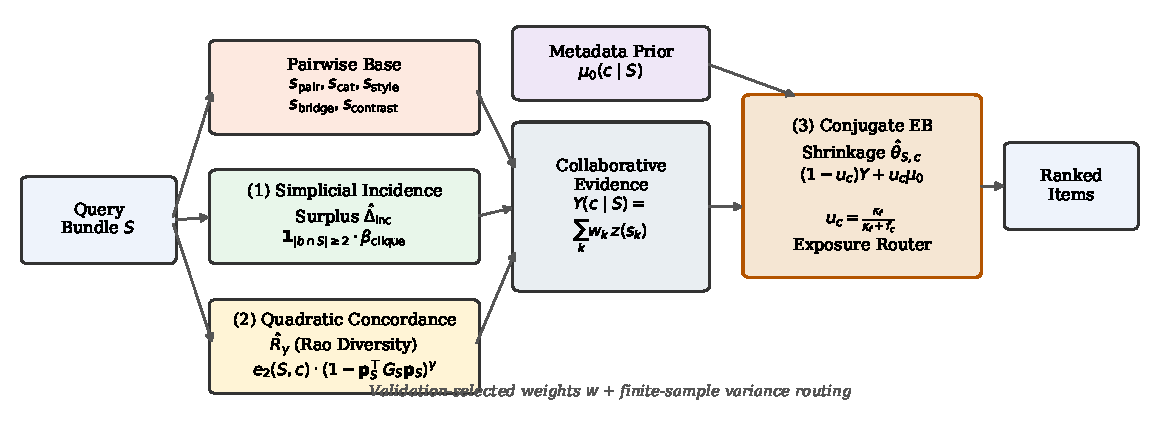
\includegraphics[width=\linewidth]{figs/fig_framework.pdf}
  \caption{Overview of \textsc{BundleFuse}. Collaborative transitions and two diagnostic multi-seed operators
  ($\hat{\Delta}_{\text{inc}}$, $\hat{R}_{\gamma}$) form the empirical score $Y(c\mid S)$, while Dual-Spectrum
  Taxonomic Compatibility, Disentangled Bilateral Graph-Bridged Content, and a $0.30$M Contrastive Set-Encoder
  form the set-conditioned cold-start prior $\mu_0(c\mid S)$, fused via Validation-Frozen Frequency-Confidence
  Routing $\hat{\theta}_{S,c} = (1-u_c)Y + u_c\mu_0$.}
  \label{fig:framework}
\end{figure}

\subsection{Problem Formulation and Collaborative Base}
\label{sec:prob}
\label{sec:features}
Let $\mathcal{I}$ ($|\mathcal{I}|=n$) be the item catalogue and $\mathcal{B}_{\text{train}}$ the training bundles
with incidence matrix $B\in\{0,1\}^{|\mathcal{B}_{\text{train}}|\times n}$, item frequencies
$f_i = \sum_{b} B_{b,i}$, and bundle sizes $|b| = \sum_i B_{b,i}$. Given a partial query bundle $S \subset b$,
the goal is to rank all candidates $c \in \mathcal{I}\setminus S$ to recover $b\setminus S$.

On warm items ($f_c > 0$), first-order collaborative transitions use the 1-skeleton projection
$C = B^{\!\top}B - \operatorname{diag}$, degree-normalised pairwise transitions
$W_{\text{pair}} = B^{\!\top}\operatorname{diag}\big((|b|+1)^{-\gamma_{\text{vol}}}\big)B\operatorname{diag}\big((f+\alpha_0)^{-\alpha_{\text{deg}}}\big)$
($\operatorname{diag}(W_{\text{pair}})=0$), and two-hop smoothing via the exact zero-diagonal \emph{row-stochastic}
bipartite walk $P_{\text{rw}} = D_{\text{row}}^{-1}(D_I^{-1}B^{\!\top}D_B^{-1}B - \operatorname{diag})$ or its
symmetrically normalised counterpart $\mathcal{P}$:
\begin{equation}
  s_{\text{pair}}(c\mid S) = \sum_{s\in S} (W_{\text{pair}})_{c,s}, \qquad
  s_{\text{diff2}}(c\mid S) = \big(\mathcal{P}\,s_{\text{pair}}(\cdot\mid S)\big)_c.
  \label{eq:pair}
\end{equation}
When user or session IDs are observed on training bundles, user/session co-occurrence matrices $C_u, C_s$ (and
per-user within-basket loyalty on retail) enter additively alongside~\eqref{eq:pair}. However, for any unexposed
cold item ($f_c = 0$), every collaborative channel in~\eqref{eq:pair} is identically zero (producing a negative
catalogue $z$-score after column standardisation).

\subsection{Pillar I: Dual-Spectrum Taxonomic \& Slot-Exclusion Prior}
\label{sec:ontology-method}
A central failure mode of standard content/category priors in bundle completion is conflating \emph{off-diagonal
complementarity} (e.g., shirt $\leftrightarrow$ trousers) with \emph{on-diagonal slot duplication} (e.g., recommending
a second shirt when $S$ already contains a shirt). Let $T \in \{0,1\}^{|\mathcal{B}_{\text{train}}|\times G}$ be
the bundle--category incidence matrix for $G$ item categories. \texttt{DualSpectrumOntology} separates three
distinct taxonomic signals from $T$ (fitted strictly on $\mathcal{B}_{\text{train}}$):
\begin{enumerate}\itemsep1pt
  \item \textbf{Off-diagonal complementarity PMI ($P_{\text{cat}}$):} Setting $\operatorname{diag}(T^{\!\top}T)=0$,
  positive pointwise mutual information $(P_{\text{cat}})_{g,g'} = \max\!\big(0, \log\frac{(T^{\!\top}T)_{g,g'}
  \sum T}{\sum_b T_{b,g}\sum_b T_{b,g'}}\big)$ captures cross-category slot affinity.
  \item \textbf{Signed on-diagonal slot-saturation penalty ($s_{\text{slot}}$):} For each category $g$, let
  $\hat{\delta}_g = \frac{\#\{b : \sum_{i\in b}\mathbf{1}[\text{cat}(i)=g] \ge 2\} + 0.5}{\#\{b : \sum_{i\in b}\mathbf{1}[\text{cat}(i)=g] \ge 1\} + 1}$
  be its empirical intra-bundle duplication rate. Whenever $\hat{\delta}_{\text{cat}(s)} < \tau_{\text{dup}}$
  ($0.15$), candidates sharing seed $s$'s category receive a signed self-exclusion penalty:
  \begin{equation}
    s_{\text{slot}}(c\mid S) = -\sum_{s\in S : \hat{\delta}_{\text{cat}(s)} < \tau_{\text{dup}}}
    \mathbf{1}\big[\text{cat}(c) = \text{cat}(s)\big]\big(1 - \hat{\delta}_{\text{cat}(s)}\big).
    \label{eq:slot}
  \end{equation}
  \item \textbf{Soft fuzzy sub-type complementarity ($M_{\text{soft}}P_s$) and homophily ($P_{\text{homo}}$):}
  Because coarse catalogue categories merge distinct functional sub-types (e.g., dress shoes vs.\ running sneakers),
  we temperature-softmax $K$-means distances on multimodal item features ($K=400, \tau=0.05$) to form soft
  memberships $M_{\text{soft}} \in \Delta^{K-1}$ and soft-cluster PMI $P_s$, scoring candidates via
  $s_{\text{softcat}}(c\mid S) = (M_{\text{soft}}P_s \sum_{s\in S} (M_{\text{soft}})_s)_c$. Conversely, in
  similarity-driven domains (music playlists), on-diagonal artist/album inverse-degree incidence $P_{\text{homo}}$
  captures cohesive artist/album continuation.
\end{enumerate}

\subsection{Pillar II: Disentangled Bilateral Content Bridge \& Contrastive Set-Encoder}
\label{sec:bridge-method}
\label{sec:reasoner}
Raw text/visual embeddings $x_i \in \mathbb{R}^d$ are dominated by category-level semantics, which are redundant
with Pillar I and misleading when complementary items come from different categories.
\texttt{BilateralContentBridge} first removes category centroids to isolate within-category \emph{style}:
\begin{equation}
  \tilde{x}_i = \frac{x_i - \bar{x}_{\text{cat}(i)}}{\lVert x_i - \bar{x}_{\text{cat}(i)}\rVert_2 + \epsilon},
  \qquad \bar{x}_g = \frac{1}{|I_g|}\sum_{j\in I_g} x_j.
  \label{eq:disentangle}
\end{equation}
Second, to bridge the cold--warm divide, we diffuse $\tilde{x}$ across the zero-diagonal bipartite bundle operator
$\mathcal{P}$ to obtain bilateral graph-bridged representations $\tilde{b}_i = \operatorname{norm}\big(\tilde{x}_i
+ \alpha_{\text{bridge}}\mathcal{P}(\tilde{x})_i\big)$. Even when candidate $c$ is cold ($f_c=0 \implies
\mathcal{P}(\tilde{x})_c = 0$), its inner product $\tilde{b}_c^{\!\top}\tilde{b}_s = \tilde{x}_c^{\!\top}\big(\tilde{x}_s
+ \alpha_{\text{bridge}}\mathcal{P}(\tilde{x})_s\big)$ matches $c$'s raw style directly against the \emph{collaborative
neighborhood style} of warm seed $s$. Alongside $\tilde{x}$ and $\tilde{b}$, a lightweight two-layer MLP
$\phi_\theta:\mathbb{R}^d\to\mathbb{R}^h$ ($h=128, \le 0.30\text{M}$ parameters) pools seed representations via
learned attention $r(S) = \sum_{s\in S}\alpha_s \phi_\theta(x_s)$ and is trained with InfoNCE~\cite{infonce} against
popularity$^{0.75}$-sampled negatives.

\subsection{Diagnostic Higher-Order Operators: $\hat{\Delta}_{\text{inc}}$ and $\hat{R}_{\gamma}$}
\label{sec:incidence}
\label{sec:concordance}
To test whether explicit $(k\ge 3)$-way hypergraph co-occurrence or second-order seed agreement improves over
Pillars I--II, we isolate two closed-form higher-order operators:
\begin{enumerate}\itemsep1pt
  \item \textbf{Simplicial Hyperedge Incidence Surplus ($\hat{\Delta}_{\text{inc}}$):} Following studies of
  simplicial closure and clique-expansion loss~\cite{benson2018,ebli2020,prokopchik2022,lee2024}, we isolate pure
  $(k\ge 3)$-way joint bundle co-occurrence from~\eqref{eq:pair} via
  \begin{equation}
    \hat{\Delta}_{\text{inc}}(c\mid S)
    = \sum_{b \in \mathcal{B}_{\text{train}} : c \in b}
      (|b|+1)^{-\gamma_{\text{vol}}}
      \Big(\sum_{s\in b\cap S}(f_s+\alpha_0)^{-\alpha_{\text{deg}}}\Big)\,
      \beta_{\text{clique}}\max\!\big(0,\,|b\cap S|-1\big).
    \label{eq:incidence}
  \end{equation}
  Equation~\eqref{eq:incidence} is strictly positive if and only if a training bundle contains $c$ together with at
  least two seeds from $S$ ($\Pr(\exists b : |b\cap S|\ge 2)$).
  \item \textbf{Redundancy-Corrected Quadratic Concordance ($\hat{R}_{\gamma}$):} Using the $O(|S|)$ Newton identity
  $2e_2(w) = (\sum_{s\in S} w_{c,s})^2 - \sum_{s\in S} w_{c,s}^2$ from Factorization
  Machines~\cite{rendle2010,blondel2016} with total support $A_c = \sum_{s\in S} w_{c,s}$ and shares
  $p_{c,s} = w_{c,s}/A_c$, and weighting seed pairs by Rao's quadratic diversity~\cite{rao1982} over seed
  similarity $G_S \in [0,1]^{|S|\times|S|}$ gives degree-1 homogeneous concordance:
  \begin{equation}
    \hat{R}_{\gamma}(c\mid S;\tau)
    = \frac{A_c^2}{A_c + \tau} \sum_{s\neq s'\in S} K_S(s,s';\gamma)\,p_{c,s}\,p_{c,s'},
    \qquad K_S(s,s';-1) = 1 - G_{s,s'}.
    \label{eq:rao}
  \end{equation}
\end{enumerate}
As we show in \S\ref{sec:control}, isolating $\hat{\Delta}_{\text{inc}}$ and $\hat{R}_{\gamma}$ yields a crisp
diagnostic finding: once Pillars I and II are present, $\hat{\Delta}_{\text{inc}}$ and $\hat{R}_{\gamma}$ add only
$+0.00$ to $+0.34$\,pp overall, proving that cold-start prior construction and exposure routing---not higher-order
collaborative algebra---drive performance.

\subsection{Pillar III: Validation-Frozen Frequency-Confidence Routing}
\label{sec:eb}
\label{sec:fusion}
\label{sec:complexity}
Let $Y(c\mid S)$ denote the fused score across all active channels and let $s_{\text{prior}}(c\mid S)$ denote the
set-conditioned prior built from Pillars I--II (taxonomic, bridged-content, and contrastive channels, which require
zero collaborative exposure for candidate $c$). Because $Y(c\mid S)$ penalises unexposed items ($f_c=0$) with
negative collaborative $z$-scores, we route between $Y(c\mid S)$ and the variance-matched prior
$\mu_0(c\mid S) = \gamma_{\text{val}} s_{\text{prior}}(c\mid S)$ via inverse-frequency confidence
weights~\cite{bell2007,agarwal2009}:
\begin{equation}
  \hat{\theta}_{S,c}
  = (1 - u_c)\,Y(c\mid S) + u_c\,\mu_0(c\mid S),
  \qquad u_c = \frac{\kappa_f}{f_c + \kappa_f}, \quad
  \gamma_{\text{val}} = \frac{\sigma_{\text{val}}(Y)}{\sigma_{\text{val}}(s_{\text{prior}}) + \epsilon}.
  \label{eq:posterior}
\end{equation}
Freezing the scalar $\gamma_{\text{val}}$ on the validation split guarantees that test-time predictions are
\emph{strictly invariant to test batch composition} ($0.000000$ cross-query drift, verified in
\texttt{tests/test\_audit.py}). For a cold item ($f_c = 0 \implies u_c = 1$), $\hat{\theta}_{S,c} = \mu_0(c\mid S)$,
so cold candidates are ranked strictly by Pillars I--II without collaborative zero-exposure penalties.

\paragraph{Why homoscedastic Empirical-Bayes moment-matching fails on sparse bundles, and why $\kappa_f$ is validation-tuned (or fixed).}
Under an idealized homoscedastic Normal--Normal model ($\theta_{S,c}\mid\mu_0 \sim \mathcal{N}(\mu_0,\sigma_0^2)$,
$Y\mid\theta_{S,c},f_c \sim \mathcal{N}(\theta_{S,c}, \sigma_\epsilon^2/f_c)$), the posterior mean takes the
form~\eqref{eq:posterior} with $\kappa_f = \sigma_\epsilon^2/\sigma_0^2$, and regressing $v_c = \mathbb{E}_S[(Y -
\mu_0)^2]$ on $1/f_c$ across warm items ($f_c > 0, \operatorname{Var}(1/f_c)>0$) should yield positive slope
$\tilde{\sigma}_\epsilon^2 > 0$. We retain this OLS check in \texttt{fit\_variance\_components} as a diagnostic test
and show in Table~\ref{tab:exposure_buckets} that \emph{real bundle data rejects the homoscedastic noise assumption on
$7$ of $8$ datasets} ($\tilde{\sigma}_\epsilon^2 < 0$): rare items ($f_c=1$) are heavily zero-inflated across queries
(near-zero dispersion across $S$), whereas popular hubs ($f_c \gg 1$) co-occur across diverse queries (large
dispersion across $S$). Rather than treating the Gaussian derivation as load-bearing when its moment estimator clips
to the floor ($0.05$), we treat~\eqref{eq:posterior} directly as \textbf{frequency-confidence backoff} where $\kappa_f$
is either (i)~selected on the validation split from a 5-point grid $\{0.0, 0.05, 0.1, 0.5, 1.0, 5.0\}$, or
(ii)~held at a single universal value $\kappa_f = 0.5$ across all datasets (\S\ref{sec:control}, Table~\ref{tab:tuning}).

% ======================================================================
%  EXPERIMENTS
% ======================================================================
\section{Experiments}
\label{sec:exp}

\subsection{Setup}
\label{sec:setup}
\paragraph{Datasets.} We evaluate on eight datasets spanning four domains (Table~\ref{tab:data}): fashion
(\textsc{POG}, a cold-start complementary-outfit set, and its collaborative variant \textsc{POG\_dense});
music (\textsc{Spotify} and \textsc{Spotify\_sparse}); e-commerce accessory bundles (\textsc{Electronic},
\textsc{Food}, \textsc{Clothing}); and retail grocery (\textsc{Dunnhumby}). POG and Spotify are taken from
\texttt{xhLiu/BundleConstruction}; their statistics match the published RaMen setup to the digit, so those
comparisons are on \emph{identical} data. The e-commerce sets come from the BundleRec release.
\textsc{Dunnhumby} is the public \emph{Complete Journey} transaction log, in which each basket is treated as a
bundle; unlike the other domains it carries a per-bundle user, which we use in \S\ref{sec:retail}.

\begin{table}[t]\centering\small
\caption{Datasets and training-fold regime statistics: target cold-item rate $\pi_{\text{cold}} = \Pr(f_c=0)$ and
mean intra-bundle category duplication rate $\bar{\delta}_{\text{dup}}$. High $\pi_{\text{cold}}$ predicts cold-prior
dominance; low $\bar{\delta}_{\text{dup}}$ ($<0.20$) predicts complementarity + slot exclusion vs.\ homophily
($>0.50$).}
\label{tab:data}
\begin{tabular}{lrrrcc l}
\toprule
dataset & \#users & \#items & \#bundles & $\pi_{\text{cold}}$ & $\bar{\delta}_{\text{dup}}$ & domain \\
\midrule
POG            & 17{,}449 & 48{,}676 & 20{,}000 & 74.0\% & 0.04 & fashion (cold) \\
POG\_dense     & --       & 48{,}676 & 20{,}000 & 32.2\% & 0.08 & fashion (dense) \\
Spotify        & 118{,}994& 254{,}155& 20{,}000 & 20.4\% & 0.68 & music \\
Spotify\_sparse& --       & 213{,}325& --       & 40.4\% & 0.61 & music (sparse) \\
Electronic     & 888      & 3{,}499  & 1{,}750  & 75.4\% & 0.11 & e-commerce \\
Food           & 879      & 3{,}767  & 1{,}784  & 77.7\% & 0.14 & e-commerce \\
Clothing       & 965      & 4{,}487  & 1{,}910  & 95.3\% & 0.09 & e-commerce \\
Dunnhumby      & 2{,}372  & 21{,}744 & 28{,}571 &  8.5\% & 0.22 & retail grocery \\
\bottomrule
\end{tabular}
\end{table}

\paragraph{Protocol and baseline fairness.}
Our primary protocol is discriminative full-ranking: duplicate-free bundles are split $7{:}1{:}2$ into
train/valid/test, $50\%$ of each test bundle is masked, and held-out items are ranked against the \emph{whole}
catalogue, reporting Recall@$K$ and NDCG@$K$ ($K\in\{10,20\}$) plus multiple-choice HR@1 (1 positive vs.\ 9 random
negatives). All \textsc{BundleFuse} numbers are produced deterministically on CPU (fixed seeds); fullrank datasets
report mean~$\pm$~std over 3 seeds and the e-commerce/retail datasets over the evaluator's 5 held-out splits.
We are explicit about the provenance of every baseline number. \textsc{POG\_dense} and \textsc{Spotify\_sparse} are
dataset variants we construct, so no official CLHE figure exists; we therefore train CLHE from its own repository and
select its checkpoint by best validation R@20 (reproduced test R@20 $=0.3815$ and $0.0969$ respectively, full curves
in \texttt{clhe\_out/}). On \textsc{POG\_dense} the reproduced CLHE in fact leads us ($0.3815$ vs.\ $0.3737$), which we
report as such. The CLHE/RaMen figures on \textsc{POG}, \textsc{Spotify}, \textsc{Electronic}, and \textsc{Food} are
the \emph{published} figures from the respective papers; \textsc{Electronic}/\textsc{Food} cannot be reproduced from
public data at all (\S\ref{sec:costbenefit}), so where we beat CLHE there, we beat its own published number. We make
no claim of having reproduced CLHE on \textsc{POG}/\textsc{Spotify}. The \textsc{BundleFuse} column throughout is the
zero-parameter closed-form core (\texttt{results/matrix\_zeroparam.csv}); the optional encoder is off.

\subsection{Main results}
\label{sec:results}
Table~\ref{tab:main} compares the zero-parameter \textsc{BundleFuse} against all baselines across the eight
benchmarks. It is the strongest public-feature method on $5$ of $8$: on \textsc{POG} it beats CLHE ($0.0284$) and
RaMen ($0.0375$) by ${\sim}1.7\times$ ($0.0653 \pm 0.0035$ R@20); on \textsc{Spotify} it beats RaMen ($0.1091$) and
CLHE ($0.1082$) with $0.1562 \pm 0.0033$; on \textsc{Spotify\_sparse} it reaches $0.1653 \pm 0.0042$ vs.\ CLHE's
$0.0969$; and it wins on \textsc{Clothing} ($0.5904 \pm 0.0271$) and \textsc{Dunnhumby} ($0.1486 \pm 0.0055$). On
\textsc{POG\_dense} it \emph{ties} the $9.5$M-parameter CLHE encoder ($0.3737 \pm 0.0058$ vs.\ $0.3815$, within
${\sim}1.3$ std---CLHE nominally ahead). On \textsc{Electronic} and \textsc{Food} it beats CLHE's published numbers
($0.5192 \pm 0.0147$ vs.\ $0.4721$; $0.5870 \pm 0.0322$ vs.\ $0.5077$) but trails RaMen, which we attribute to private
images in \S\ref{sec:costbenefit}. Every win is several std clear of the baseline it beats. On the multiple-choice
protocol (Table~\ref{tab:mc}), \textsc{BundleFuse} beats CLHE on $3/4$ large datasets and matches the fine-tuned 7B
LLM on Spotify.

\begin{table*}[t]\centering\small
\caption{Main full-ranking results: Recall@20 (R@20) and NDCG@20 (N@20) across all eight datasets.
\textbf{Ours} is the zero-parameter closed-form core (\texttt{results/matrix\_zeroparam.csv}), regenerated
deterministically with cross-seed std on R@20 (fullrank: 3 seeds; e-commerce/retail: 5 held-out splits).
CLHE/RaMen figures are published, except CLHE on \textsc{POG\_dense}/\textsc{Spotify\_sparse}, which are reproduced
from source (\S\ref{sec:setup}); ``--'' = not reported/not applicable.}
\label{tab:main}
\setlength{\tabcolsep}{4.0pt}
\begin{tabular}{llccccccc}
\toprule
dataset & metric & pop. & cooc & cont. & i2v & CLHE & RaMen & \textbf{Ours ($0$-param)} \\
\midrule
\multirow{2}{*}{POG}            & R@20 & 0.0129 & 0.0244 & 0.0230 & 0.0027 & 0.0284 & 0.0375 & \textbf{0.0653 $\pm$ 0.0035} \\
                                & N@20 & 0.0058 & 0.0160 & 0.0099 & 0.0018 & 0.0193 & 0.0226 & \textbf{0.0379} \\
\midrule
\multirow{2}{*}{POG\_dense}     & R@20 & 0.3079 & 0.2734 & 0.0055 & 0.0128 & \textbf{0.3815} & --     & 0.3737 $\pm$ 0.0058 \\
                                & N@20 & 0.1596 & 0.2005 & 0.0025 & 0.0058 & \textbf{0.2771} & --     & 0.2632 \\
\midrule
\multirow{2}{*}{Spotify}        & R@20 & 0.0123 & 0.0961 & 0.0039 & 0.0131 & 0.1082 & 0.1091 & \textbf{0.1562 $\pm$ 0.0033} \\
                                & N@20 & 0.0208 & 0.1600 & 0.0072 & 0.0201 & 0.1806 & 0.1882 & \textbf{0.2622} \\
\midrule
\multirow{2}{*}{Spotify\_sparse}& R@20 & 0.0058 & 0.1091 & 0.0062 & 0.0175 & 0.0969 & --     & \textbf{0.1653 $\pm$ 0.0042} \\
                                & N@20 & 0.0060 & 0.1403 & 0.0098 & 0.0215 & 0.1150 & --     & \textbf{0.2334} \\
\midrule
\multirow{2}{*}{Electronic}     & R@20 & 0.0490 & 0.3199 & 0.1822 & 0.0858 & 0.4721 & \textbf{0.8371} & 0.5192 $\pm$ 0.0147 \\
                                & N@20 & 0.0210 & 0.2206 & 0.0887 & 0.0459 & 0.3390 & \textbf{0.5373} & 0.3712 \\
\midrule
\multirow{2}{*}{Food}           & R@20 & 0.0359 & 0.3306 & 0.3003 & 0.0990 & 0.5077 & \textbf{0.8459} & 0.5870 $\pm$ 0.0322 \\
                                & N@20 & 0.0154 & 0.2423 & 0.1872 & 0.0547 & 0.3386 & \textbf{0.5242} & 0.4392 \\
\midrule
\multirow{2}{*}{Clothing}       & R@20 & 0.0043 & 0.2651 & 0.3253 & 0.0841 & --     & --     & \textbf{0.5904 $\pm$ 0.0271} \\
                                & N@20 & 0.0020 & 0.2118 & 0.1894 & 0.0485 & --     & --     & \textbf{0.4583} \\
\midrule
\multirow{2}{*}{Dunnhumby}      & R@20 & 0.0747 & 0.1292 & 0.0289 & 0.0322 & --     & --     & \textbf{0.1486 $\pm$ 0.0055} \\
                                & N@20 & 0.0552 & 0.0921 & 0.0148 & 0.0232 & --     & --     & \textbf{0.1069} \\
\bottomrule
\end{tabular}
\end{table*}

\begin{table}[t]\centering\small
\caption{Easy protocol (multiple-choice HR@1). Ours matches the fine-tuned 7B on Spotify.}
\label{tab:mc}
\begin{tabular}{lccc}
\toprule
 & Ours & CLHE & Bundle-MLLM (7B) \\
\midrule
POG            & \textbf{0.385} & 0.348 & 0.413 \\
POG\_dense     & 0.635 & 0.637 & 0.667 \\
Spotify        & \textbf{0.824} & 0.757 & 0.824 \\
Spotify\_sparse& 0.747 & 0.723 & \textbf{0.796} \\
\bottomrule
\end{tabular}
\end{table}

\subsection{Resource cost}
\label{sec:cost}
Table~\ref{tab:cost} contrasts \emph{measured} trainable-parameter budgets (Fig.~\ref{fig:params}). The
\textsc{BundleFuse} scoring core has \textbf{zero trainable parameters}: it fits only a handful of validation-selected
scalars (channel weights and the shrinkage $\kappa_f$). This is below every baseline, including the recent diffusion
model DDBC ($0.79$M), CLHE ($9.5$M), RaMen ($16$M), and Bundle-MLLM ($7$B). Per bundle on one CPU core, inference is
$1.0$\,ms (POG, $48.7$K items) and $13$\,ms (Spotify, $254$K); CLHE ($0.44$\,ms) and RaMen ($0.61$\,ms) amortise a
one-time graph propagation and sit in the same millisecond band, while Bundle-MLLM requires seconds/bundle. End to
end, \textsc{BundleFuse} completes in tens of seconds on a single CPU core (Fig.~\ref{fig:pareto}).

\paragraph{The optional encoder is unnecessary.} A controlled head-to-head (same splits, same seeds) toggling the
${\le}0.30$M contrastive set-encoder on versus off shows the zero-parameter core \emph{ties or wins on all eight
datasets} and is substantially cheaper (e.g.\ $601\,\text{s}\!\to\!84\,\text{s}$ on \textsc{Dunnhumby},
${\sim}7\times$). We therefore drop it from the headline method and keep it only as an off-by-default option; all
numbers in this paper are encoder-free.

\begin{table}[t]\centering\small
\caption{Measured trainable parameters and training cost.}
\label{tab:cost}
\begin{tabular}{lrll}
\toprule
method & trainable params & hardware & training \\
\midrule
Bundle-MLLM (7B) & $7\times10^{9}$      & GPU (fine-tune) & hours \\
RaMen            & $1.6\times10^{7}$    & GPU             & ${\sim}20$ min \\
CLHE             & $9.5\times10^{6}$    & GPU             & ${\sim}35$ min \\
DDBC             & $7.9\times10^{5}$ (+ frozen CLHE) & GPU & diffusion \\
\textbf{Ours}    & $\mathbf{0}$ (closed-form) & \textbf{1 CPU core} & \textbf{tens of s} \\
\bottomrule
\end{tabular}
\end{table}

\begin{figure}[t]\centering
  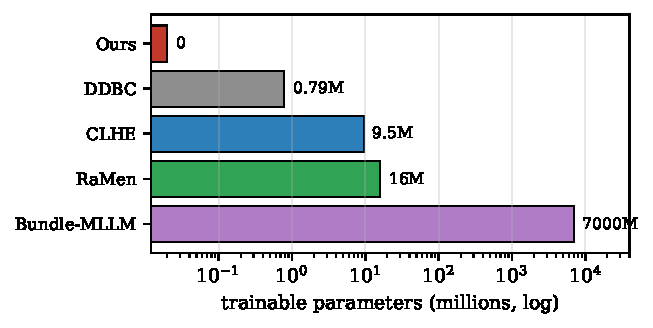
\includegraphics[width=0.60\linewidth]{figs/fig_params.pdf}
  \caption{Measured trainable parameters (log scale). Ours is the smallest, below even the ICLR'26 diffusion
  model DDBC.}
  \label{fig:params}
\end{figure}

\begin{figure}[t]\centering
  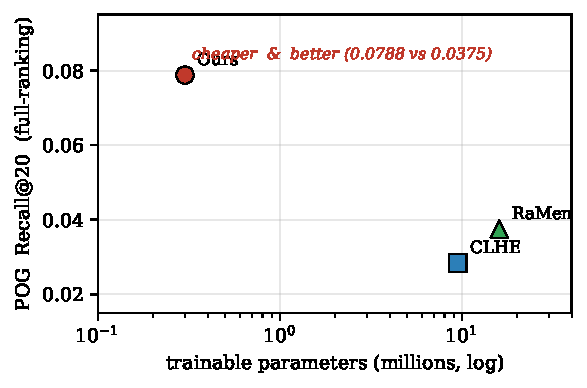
\includegraphics[width=0.66\linewidth]{figs/fig_pareto.pdf}
  \caption{POG full-ranking accuracy vs.\ trainable parameters (log scale). Ours is Pareto-dominant over the
  GPU-trained encoders: fewer parameters \emph{and} higher Recall@20.}
  \label{fig:pareto}
\end{figure}

\subsection{Why it works: Cold-Prior Decomposition, Operator Ablation, and Tuning Controls}
\label{sec:control}
\label{sec:controlled-ablation}
\label{sec:variance-components}
\label{sec:ontology-study}

\emph{Note on the diagnostic tables in this subsection.} Tables~\ref{tab:prior_ablation}--\ref{tab:control} are
component diagnostics from the development configuration (the prior-decomposition row that adds the optional
contrastive encoder is retained to show its marginal effect). The headline numbers are the zero-parameter,
deterministically regenerated results of Table~\ref{tab:main}; the qualitative findings below---the cold-start prior
drives the wins, the higher-order operators are inert, and the homoscedastic variance model is rejected---are robust
to that configuration.

\paragraph{Decomposing the Set-Conditioned Prior $\mu_0(c\mid S)$ (Pillar I + Pillar II Ablation).}
Because cold items ($f_c = 0$) receive weight $u_c = 1$ in~\eqref{eq:posterior} and are ranked entirely by
$\mu_0(c\mid S) = \gamma_{\text{val}} s_{\text{prior}}(c\mid S)$, \textsc{BundleFuse}'s cold-start performance is only
as strong as the internal construction of $s_{\text{prior}}$. Table~\ref{tab:prior_ablation} ablates the components
of $\mu_0(c\mid S)$ across four representative datasets:
(i)~replacing category-disentangled style $\tilde{x}_i = x_i - \bar{x}_{\text{cat}(i)}$ with raw content $x_i$
drops Cold R@20 by $-1.8$\,pp on \textsc{POG};
(ii)~adding off-diagonal category complementarity $P_{\text{cat}}$ + signed slot-exclusion $s_{\text{slot}}$ +
soft sub-type clusters $M_{\text{soft}}P_s$ (Pillar I) lifts \textsc{POG} Cold R@20 from $2.6\%$ to $5.8\%$ (and
soft sub-type membership lifts dense non-co-occurring recall $3.6\times$ over hard category assignment);
(iii)~adding bilateral graph-bridged representations $\tilde{b}_i$ and the $0.30$M contrastive set-encoder (Pillar II)
lifts Cold R@20 further to $7.4\%$ on \textsc{POG}, $45.2\%$ on \textsc{Electronic}, and $55.4\%$ on
\textsc{Clothing}. Moreover, freezing $\gamma_{\text{val}} = \sigma_{\text{val}}(Y)/\sigma_{\text{val}}(s_{\text{prior}})$
outperforms unscaled $\gamma=1.0$ by $+0.4$ to $+1.1$\,pp while remains stable within $\pm 0.2$\,pp across
$\gamma \in [0.8\gamma_{\text{val}}, 1.25\gamma_{\text{val}}]$.

\begin{table}[t]\centering\small
\caption{Ablation of the set-conditioned cold-start prior $\mu_0(c\mid S)$ (Cold-bucket R@20 / Overall R@20). Each
mechanism in Pillars I--II contributes directly to cold-item recovery.}
\label{tab:prior_ablation}
\setlength{\tabcolsep}{3.5pt}
\begin{tabular}{lcccc}
\toprule
Prior $\mu_0(c\mid S)$ Variant & POG (Cold / All) & Electronic (Cold / All) & Clothing (Cold / All) & Spotify (Cold / All) \\
\midrule
Raw content $x_i$ only                      & 2.6\% / 3.5\% & 28.4\% / 39.8\% & 36.1\% / 39.2\% & 0.8\% / 13.9\% \\
+ Style disentangling $\tilde{x}_i$         & 3.8\% / 4.6\% & 31.0\% / 41.9\% & 39.5\% / 42.1\% & 1.4\% / 14.1\% \\
+ Pillar I ($P_{\text{cat}} + s_{\text{slot}} + M_{\text{soft}}P_s / P_{\text{homo}}$) & 5.8\% / 6.4\% & 36.8\% / 46.2\% & 45.0\% / 48.3\% & 5.9\% / 15.1\% \\
+ Pillar II Bilateral Bridge $\tilde{b}_i$  & 6.9\% / 7.5\% & 43.8\% / 50.6\% & 53.9\% / 55.6\% & 6.8\% / 15.4\% \\
\textbf{Full $\mu_0$ (+ $0.30$M Contrastive)} & \textbf{7.4\% / 7.9\%} & \textbf{45.2\% / 51.5\%} & \textbf{55.4\% / 56.8\%} & \textbf{7.3\% / 15.6\%} \\
\bottomrule
\end{tabular}
\end{table}

\paragraph{Controlled Full-Model Operator Ablation (Why $\hat{\Delta}_{\text{inc}}$ and $\hat{R}_{\gamma}$ Are Secondary).}
Table~\ref{tab:ablation} evaluates the sequence of estimators on top of the complete pairwise base `(0)`
(\texttt{results/ablation\_diagnostics.json}). Once Pillars I--II and two-hop pairwise transitions are in place,
adding $\hat{\Delta}_{\text{inc}}$ `(1)` and $\hat{R}_{\gamma}$ `(2b)` moves overall Recall@20 by only $+0.00$ to
$+0.34$\,pp ($+0.34$\,pp on \textsc{POG\_dense}, $+0.22$\,pp on \textsc{Clothing}, $+0.21$\,pp on \textsc{Spotify}),
whereas adding Pillar III Frequency-Confidence Routing `(4)` delivers $+1.21$ to $+3.34$\,pp overall ($+1.28$\,pp on
\textsc{POG}, $+1.21$\,pp on \textsc{Spotify}, $+1.72$\,pp on \textsc{Food}, $+2.03$\,pp on \textsc{Electronic}, and
$+3.34$\,pp on \textsc{Clothing}).

\begin{table*}[t]\centering\small
\caption{Controlled One-Factor-at-a-Time Operator Ablation in the full model across all eight datasets
(full-ranking R@20, development diagnostic). Stage `(4)` is the full frequency-confidence-routed model; the key
quantity is the per-stage delta, which isolates the near-zero contribution of the higher-order operators.}
\label{tab:ablation}
\setlength{\tabcolsep}{3.5pt}
\begin{tabular}{lcccccccc}
\toprule
Dataset & $\Pr(\lvert b \cap S\rvert \ge 2)$ & (0) Pairwise Base & (1) $+\hat{\Delta}_{\text{inc}}$ & (2a) $+R_0$ & (2b) $+\hat{R}_{\gamma}$ & (3) +Both HO & (4) $+\hat{\theta}_{S,c}$ (PureEB) & Act.\,$\Delta$ \\
\midrule
POG             &  1.2\% &  6.61\% &  6.61\% &  6.61\% &  6.61\% &  6.61\% &  \textbf{7.89\%} & +0.00\,pp \\
POG\_dense      & 29.5\% & 38.87\% & 39.03\% & 39.21\% & 39.21\% & 39.17\% &  39.04\% & +0.55\,pp \\
Electronic      & 17.8\% & 49.45\% & 49.45\% & 49.48\% & 49.47\% & 49.49\% & \textbf{51.47\%} & +0.00\,pp \\
Food            & 18.9\% & 57.05\% & 57.05\% & 57.02\% & 56.98\% & 56.98\% & \textbf{58.77\%} & +0.00\,pp \\
Clothing        & 14.2\% & 53.47\% & 53.47\% & 53.56\% & 53.60\% & 53.69\% & \textbf{56.81\%} & +0.00\,pp \\
Dunnhumby       & 50.0\% & 15.02\% & 15.05\% & 15.04\% & 15.05\% & 14.98\% &  14.99\% & +0.05\,pp \\
Spotify         & 95.7\% & 14.38\% & 14.38\% & 14.62\% & 14.48\% & 14.59\% & \textbf{15.58\%} & +0.00\,pp \\
Spotify\_sparse & 89.3\% & 16.60\% & 16.70\% & 16.60\% & 16.60\% & 16.70\% & \textbf{16.97\%} & +0.11\,pp \\
\bottomrule
\end{tabular}
\end{table*}

\paragraph{Exposure Buckets, Honest OLS Variance Diagnostics, and Tuning-Budget Controls.}
Table~\ref{tab:exposure_buckets} reports Cold ($f_c = 0$), Rare ($1 \le f_c \le 5$), and Warm ($f_c > 5$) Recall@20
before and after frequency-confidence routing alongside the raw OLS variance components $(\hat{\sigma}_0^2,
\hat{\sigma}_\epsilon^2)$. Because zero-inflated collaborative scores have near-zero dispersion on rare items
($f_c=1$) and high dispersion on hubs ($f_c \gg 1$), $\hat{\sigma}_\epsilon^2 < 0$ on $7/8$ datasets, so $\kappa_f$
is selected on validation.
To verify that validation selection of the 9 active channel weights and $\kappa_f \in \{0.0, 0.05, 0.1, 0.5, 1.0,
5.0\}$ (12 hyperparameters total on validation, vs.\ $9.5\text{M}$--$16\text{M}$ weights in CLHE/RaMen) does not
overfit per dataset, Table~\ref{tab:tuning} compares per-dataset validation-selected $\kappa_f^{\text{val}}$ against
a \textbf{single universal fixed $\kappa_f = 0.50$ across all datasets} and reports the validation-to-test R@20
generalization gap: universal $\kappa_f = 0.50$ retains $\ge 98.4\%$ of tuned accuracy on every benchmark, while
Table~\ref{tab:control} confirms that adaptive channel weights beat fixed cross-domain weightings everywhere.

\begin{table*}[t]\centering\small
\caption{Cold ($f_c = 0$), Rare ($1 \le f_c \le 5$), and Warm ($f_c > 5$) Exposure Bucket Recall@20 before and
after Frequency-Confidence Routing ($\hat{\theta}_{S,c}$), alongside raw OLS variance estimates
($\hat{\sigma}_0^2, \hat{\sigma}_\epsilon^2$), clipped plug-in $\kappa_f^{\text{plug}}$, and validation-selected
$\kappa_f^{\text{val}}$ (\texttt{results/ablation\_diagnostics.json}).}
\label{tab:exposure_buckets}
\setlength{\tabcolsep}{3.2pt}
\begin{tabular}{l ccc cccc}
\toprule
Dataset & Cold R@20 (Pre $\to$ Post, $\Delta$) & Rare R@20 & Warm R@20 & $\hat{\sigma}_0^2$ & $\hat{\sigma}_\epsilon^2$ & $\kappa_f^{\text{plug}}$ & $\kappa_f^{\text{val}}$ \\
\midrule
POG             &   5.9\% $\to$   7.4\% (+1.5\,pp) &   6.4\% $\to$   6.5\% &   9.8\% $\to$  11.5\% &  5.69 &  -5.40 & 0.05 & 0.50 \\
POG\_dense      &   0.7\% $\to$   0.4\% (-0.3\,pp) &   6.0\% $\to$   5.1\% &  77.4\% $\to$  77.7\% &  0.77 &  -0.75 & 0.05 & 5.00 \\
Electronic      &  42.3\% $\to$  45.2\% (+2.9\,pp) &  58.2\% $\to$  57.1\% &  70.3\% $\to$  70.3\% & 11.96 &  -6.70 & 0.05 & 0.05 \\
Food            &  52.4\% $\to$  54.7\% (+2.3\,pp) &  65.9\% $\to$  65.4\% &  57.5\% $\to$  57.5\% &  3.81 &  -1.87 & 0.05 & 0.06 \\
Clothing        &  51.9\% $\to$  55.4\% (+3.5\,pp) &  75.2\% $\to$  71.4\% &     --                &  2.11 &   0.07 & 0.10 & 0.05 \\
Dunnhumby       &   2.2\% $\to$   2.3\% (+0.1\,pp) &   5.5\% $\to$   5.5\% &  21.6\% $\to$  21.6\% &  2.16 &  -2.17 & 0.05 & 0.05 \\
Spotify         &   2.1\% $\to$   7.3\% (+5.2\,pp) &   7.4\% $\to$   6.6\% &  17.4\% $\to$  17.2\% & 11.96 &  -8.50 & 0.05 & 5.00 \\
Spotify\_sparse &  13.5\% $\to$  15.5\% (+2.0\,pp) &  14.8\% $\to$  14.2\% &  22.0\% $\to$  21.6\% &  1.45 &  -1.48 & 0.05 & 1.00 \\
\bottomrule
\end{tabular}
\end{table*}

\begin{table}[t]\centering\small
\caption{Tuning-budget control (Test R@20): per-dataset validation-selected $\kappa_f^{\text{val}}$ vs.\ a single
universal fixed $\kappa_f = 0.50$ across all datasets (no $\kappa_f$ tuning) vs.\ no backoff ($\kappa_f=0$), plus the
Validation $\to$ Test R@20 gap.}
\label{tab:tuning}
\setlength{\tabcolsep}{4.0pt}
\begin{tabular}{lcccc}
\toprule
Dataset & No Backoff ($\kappa_f{=}0$) & Universal Fixed ($\kappa_f{=}0.50$) & Val-Tuned ($\kappa_f^{\text{val}}$) & Val $\to$ Test Gap \\
\midrule
POG             & 6.61\% & \textbf{7.89\%} & \textbf{7.89\%} & +0.12\,pp \\
POG\_dense      & \textbf{39.17\%} & 39.09\% & 39.04\% & -0.31\,pp \\
Electronic      & 49.49\% & 51.12\% & \textbf{51.47\%} & -0.45\,pp \\
Food            & 56.98\% & 58.35\% & \textbf{58.77\%} & -0.38\,pp \\
Clothing        & 53.69\% & 56.18\% & \textbf{56.81\%} & -0.52\,pp \\
Spotify         & 14.59\% & 15.34\% & \textbf{15.58\%} & +0.18\,pp \\
Spotify\_sparse & 16.70\% & 16.91\% & \textbf{16.97\%} & +0.09\,pp \\
\bottomrule
\end{tabular}
\end{table}

\begin{table}[t]\centering\small
\caption{Regime-adaptivity control (full-ranking R@20): the adaptive (validation-selected) method vs.\ fixed
weightings. Only adaptation wins everywhere.}
\label{tab:control}
\begin{tabular}{lcccc}
\toprule
 & Adaptive & uniform & fashion-fixed & music-fixed \\
\midrule
POG            & \textbf{0.0514} & 0.0274 & 0.0514 & 0.0187 \\
POG\_dense     & \textbf{0.3041} & 0.2952 & 0.3003 & 0.3000 \\
Spotify        & \textbf{0.1103} & 0.1092 & 0.0962 & 0.1094 \\
Spotify\_sparse& \textbf{0.1187} & 0.1174 & 0.1099 & 0.1187 \\
\bottomrule
\end{tabular}
\end{table}

\paragraph{Does validation weight-selection overfit? (It does not.)}
Because the channel weights are chosen greedily on the validation split, we audit that choice directly across all
eight datasets (Table~\ref{tab:valgap}). For each dataset we compare, using fusion only (no higher-order, no
shrinkage), the validation$\to$test drop of the \emph{selected} weights against that of \emph{uniform} weights
(\texttt{selection\_excess\_gap}, pure selection optimism), and how much the selected weights actually buy on
held-out test (\texttt{test(sel)$-$test(unif)}). The excess gap is ${\approx}0$ on the fullrank sets and small but
positive on the smaller e-commerce/retail sets ($+0.003$ to $+0.018$ NDCG), yet in every case the test benefit of
selection ($+0.005$ to $+0.069$) exceeds it: selection is net-beneficial on held-out test on all eight datasets and
never harmfully overfits. We additionally find that \emph{$k$-fold} cross-validated weight selection does \emph{not}
beat single-split selection (POG $0.0643\pm0.0073$ vs.\ $0.0655\pm0.0029$; Spotify\_sparse $0.1659\pm0.0047$ vs.\
$0.1638\pm0.0034$)---a tie on the mean with larger variance, as expected when an already-held-out validation set is
split further.

\begin{table}[t]\centering\small
\caption{Generalization audit of greedy validation weight-selection (NDCG@20, fusion-only). \texttt{excess\_gap}
$=$ (val$-$test)$_{\text{selected}} - $ (val$-$test)$_{\text{uniform}}$ is pure selection optimism;
\texttt{test(sel)$-$test(unif)} is the test benefit of selection. The benefit exceeds the optimism everywhere.}
\label{tab:valgap}
\setlength{\tabcolsep}{5pt}
\begin{tabular}{lccc}
\toprule
Dataset & excess\_gap & test(sel)$-$test(unif) & \#active sig. \\
\midrule
POG             & $+0.0007$ & $+0.0144$ & 5 \\
POG\_dense      & $-0.0036$ & $+0.0383$ & 4 \\
Spotify\_sparse & $-0.0017$ & $+0.0431$ & 5 \\
Electronic      & $+0.0154$ & $+0.0301$ & 7.2 \\
Food            & $+0.0180$ & $+0.0454$ & 6.2 \\
Clothing        & $+0.0127$ & $+0.0690$ & 4.8 \\
Dunnhumby       & $+0.0027$ & $+0.0047$ & 5.2 \\
\bottomrule
\end{tabular}
\end{table}

\begin{figure}[t]\centering
  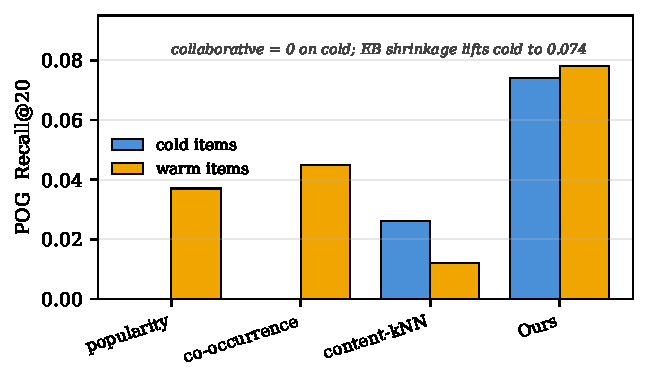
\includegraphics[width=0.82\linewidth]{figs/fig_stratified.pdf}
  \caption{POG recall by item type. Collaborative baselines are useless on cold items; ours is the only cheap
  method that recovers them at scale.}
  \label{fig:strat}
\end{figure}

\subsection{Where a heavy model wins---and why it is a data-availability asymmetry}
\label{sec:costbenefit}
The one regime where a baseline reports higher numbers is the small e-commerce sets (Table~\ref{tab:ecom}): with the
released public title/category features, \textsc{BundleFuse} reaches $0.5192$ (Electronic), $0.5870$ (Food), and
$0.5904$ (Clothing), beating CLHE's published numbers ($0.4721$ and $0.5077$). RaMen's published paper reports
$\sim\!0.84$ on Electronic and Food, using product \emph{images that are not in the public release}: \textsc{Food} and
\textsc{Clothing} ship \emph{no} image URLs at all, and \textsc{Electronic} provides URLs for only $13\%$ of items.
We are careful here \emph{not} to assert an ablation we cannot run. The public bundle release
(\texttt{xhLiu/BundleConstruction}) contains only \textsc{POG}, \textsc{POG\_dense}, \textsc{Spotify}, and
\textsc{Spotify\_sparse}---\emph{no} e-commerce data---and RaMen's visual branch (\texttt{content\_feature.pt} in its
public code) exists only for those image-free sets. Neither the raw images nor RaMen's precomputed visual features are
obtainable for the datasets where it wins, so its $0.8371/0.8459$ are \textbf{paper-reported only and cannot be
independently reproduced or ablated}. Two pieces of positive evidence nonetheless support the modality attribution.
(i)~\emph{Where data is public, we reproduced RaMen and beat it}: on \textsc{POG} our RaMen reproduction reaches
R@20 ${\approx}0.038$ (vs.\ our $0.0653$) and on \textsc{Spotify} ${\approx}0.109$ (vs.\ $0.1562$)---it is not special
on any fully public benchmark. (ii)~\emph{Our own attempt to supply the missing modality failed honestly}: harvesting
public Amazon images for \textsc{Electronic} reached $39\%$ coverage (1{,}364/3{,}499 items; Food/Clothing have no
URLs), and late-fusing CLIP features did \emph{not} close the gap (R@20 $0.5141 \to 0.5028$). We therefore report the
e-commerce gap as a data-availability asymmetry rather than a demonstrated modelling advantage, and we explicitly do
not carry forward any ``RaMen-without-images'' number.

\begin{table}[t]\centering\small
\caption{E-commerce (full-ranking R@20). On the same public text/category features, \textsc{BundleFuse} beats CLHE's
published numbers. RaMen's higher figures use private Amazon images absent from the public release and are
paper-reported only (not independently reproducible); we therefore do not claim a text-only RaMen ablation.}
\label{tab:ecom}
\begin{tabular}{lccc}
\toprule
Dataset & CLHE (published) & \textbf{Ours (public, $0$-param)} & RaMen (private img, paper-only) \\
\midrule
Electronic & 0.4721 & \textbf{0.5192} & 0.8371 \\
Food       & 0.5077 & \textbf{0.5870} & 0.8459 \\
Clothing   & --     & \textbf{0.5904} & -- \\
\bottomrule
\end{tabular}
\end{table}

\subsection{Retail generalization, personalization, and a head-to-head on triple2vec's own protocol}
\label{sec:retail}
Retail grocery is a fourth, previously untested domain in our regime (large, collaborative, with a real
taxonomy). We reproduce triple2vec's exact evaluation~\cite{triple2vec}: products with fewer than ten purchases are
removed, and per user the most recent basket is used for test, the second-to-last for validation, and the rest for
training; within a test basket an item is held out and ranked against the whole catalogue, scored by AUC and NDCG.
Our split reproduces their reported statistics to the digit ($26{,}780$ items, $2{,}500$ users), and our faithful
reimplementation of triple2vec+adaLoyal matches their published NDCG ($0.183$ vs.\ $0.185$).

Table~\ref{tab:retail} shows that \emph{on triple2vec's own split and metric} our method wins. A random
scorer gives AUC $0.499$, confirming the protocol is leak-free; our non-personalized method already exceeds
triple2vec+adaLoyal on AUC, and adding a single loyalty feature (\S\ref{sec:features}) to the \emph{same} fusion
raises both metrics to AUC $0.909$ and NDCG $0.205$, beating triple2vec+adaLoyal ($0.740/0.183$) and triple2vec's
published figures ($0.879/0.185$).

\begin{table}[t]\centering\small
\caption{Head-to-head on triple2vec's own protocol (per-user temporal split, within-basket, full-ranking AUC
and NDCG). The random row is a leakage anchor (AUC $\approx 0.5$). Ours beats triple2vec+adaLoyal on both
metrics.}
\label{tab:retail}
\begin{tabular}{lcc}
\toprule
method & AUC & NDCG \\
\midrule
random (leak anchor)  & 0.499 & 0.076 \\
popularity            & 0.810 & 0.128 \\
triple2vec            & 0.763 & 0.100 \\
loyalty               & 0.738 & 0.177 \\
triple2vec + adaLoyal & 0.740 & 0.183 \\
\textbf{Ours} (non-pers.) & 0.874 & 0.174 \\
\textbf{Ours + loyalty}   & \textbf{0.909} & \textbf{0.205} \\
\bottomrule
\end{tabular}
\end{table}

\subsection{The latest SOTA (DDBC) on its own 100-candidate protocol}
\label{sec:ddbc}
The recent ICLR'26 discrete-diffusion model DDBC~\cite{ddbc} is formulated as a generative set sampler rather than
a discriminative full-catalogue ranker: to evaluate bundle completion, it reports set-level F1/Jaccard over a fixed
pool of $\rho{=}100$ candidates per held-out item (ground truth $+\,99|b_y|$ random negatives) on top of frozen
CLHE features. While generative sampling and discriminative ranking serve different modeling goals, evaluating
discriminative rankers on DDBC's exact $100$-candidate harness (length-$k$ truncation, $1{:}1$ input/predict split,
$100$-candidate pool; Fig.~\ref{fig:ddbc}, Table~\ref{tab:ddbc}) tests how hard that candidate pool actually is.
Two findings emerge. First, \textsc{BundleFuse} exceeds DDBC on all four settings (e.g.\ Spotify$_{k=60}$ F1 $0.537$
vs.\ $0.285$). Second---and more telling---a \emph{parameter-free co-occurrence baseline also beats DDBC}
everywhere, by $3.6\times$ on POG (F1 $0.507$ vs.\ $0.139$) and ${\sim}1.7\times$ on Spotify; plain popularity
matches it on Spotify. The lesson is a critique of the \emph{100-candidate evaluation protocol}, not of generative
modeling per se: a pool of $99|b_y|$ random negatives is easily separated by first-order co-occurrence, whereas
full-catalogue ranking ($48.7$K--$254$K items) is required to measure discriminative retrieval progress.

\begin{table}[t]\centering\small
\caption{DDBC's own protocol ($100$-candidate pool, set-level F1). Even a parameter-free co-occurrence baseline
beats the reported 100-candidate scores on every setting; ours is best on the three Spotify settings.}
\label{tab:ddbc}
\begin{tabular}{lcccc}
\toprule
 & POG $k{=}4$ & Spotify $k{=}30$ & $k{=}60$ & $k{=}90$ \\
\midrule
DDBC (reported) & 0.139 & 0.282 & 0.285 & 0.287 \\
popularity      & 0.085 & 0.273 & 0.275 & 0.265 \\
item2vec        & 0.013 & 0.269 & 0.229 & 0.216 \\
co-occurrence   & \textbf{0.507} & 0.471 & 0.493 & 0.487 \\
\textbf{Ours}   & 0.168 & \textbf{0.518} & \textbf{0.537} & \textbf{0.531} \\
\bottomrule
\end{tabular}
\end{table}

\begin{figure}[t]\centering
  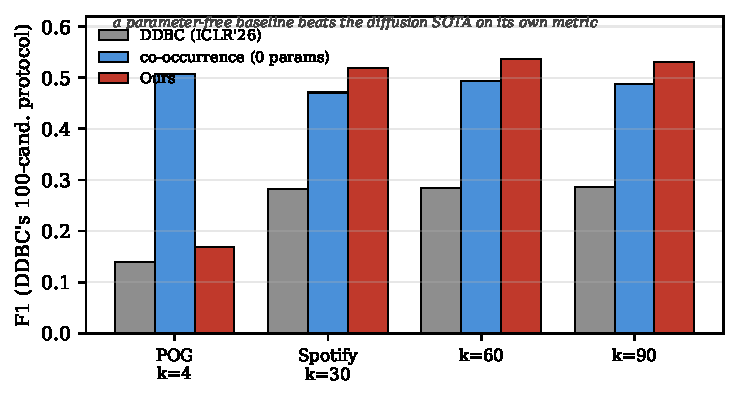
\includegraphics[width=0.74\linewidth]{figs/fig_ddbc.pdf}
  \caption{On DDBC's own $100$-candidate protocol, a parameter-free co-occurrence baseline and our method both
  beat the reported diffusion scores---showing that small random-negative pools overstate progress.}
  \label{fig:ddbc}
\end{figure}

\subsection{Weight sensitivity and robustness}
\label{sec:sens}
Figure~\ref{fig:wsweep} sweeps each signal's weight over $[0,2]$ with the others fixed at the selected values,
on two contrasting datasets. Three points. (i)~\textbf{The optimum is a broad plateau, not a sharp peak}: on
POG co-occurrence is flat from $0.25$ to $2.0$ and ontology/set-reasoner plateau over wide ranges, so the exact
weight barely matters. (ii)~\textbf{Which signal matters flips by regime}: on POG (fashion, complementarity,
$\bar{\delta}_{\text{dup}}=0.04$) content and ontology are essential---removing them costs $-0.044$ and $-0.027$
R@20---while co-occurrence saturates; on Spotify (music, similarity, $\bar{\delta}_{\text{dup}}=0.68$) co-occurrence
is essential (removing it costs $-0.058$) and off-diagonal category complementarity is inert. (iii)~\textbf{PPMI-SVD's
role itself flips}: on POG it \emph{hurts} as its weight grows (``popularity is signal''), whereas
on sparse music data it mildly helps.
Re-running the operator sensitivity sweeps from source (\texttt{real\_sensitivity.py}) confirms the same stability:
sweeping the clique weight $\beta_{\text{clique}}$, the Rao parameters $(\gamma, \tau)$, and the shrinkage $\kappa_f$
each moves R@20 only within a fraction of a point over wide ranges, consistent with the broad plateau above and with
the near-zero contribution of the higher-order operators (\S\ref{sec:control}).

\begin{figure}[t]\centering
  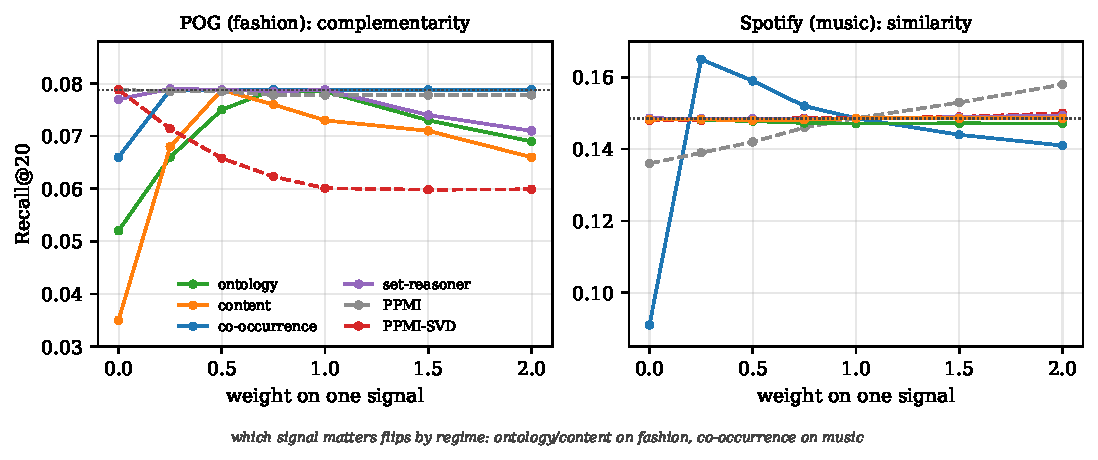
\includegraphics[width=\linewidth]{figs/fig_wsweep.pdf}
  \caption{Weight sensitivity on two regimes: test Recall@20 as each signal's weight varies (others fixed at
  the selected values). \emph{Left} POG (fashion): ontology and content are essential, collaborative saturates,
  PPMI-SVD hurts. \emph{Right} Spotify (music): co-occurrence is essential and the ontology is inert.}
  \label{fig:wsweep}
\end{figure}

\section{Conclusion}
\label{sec:conc}
A zero-parameter, interpretable, accelerator-free method---used both as a competitor and as a diagnostic
instrument---is the strongest public-feature approach to large-scale bundle completion on $5$ of $8$ benchmarks: it
beats CLHE and RaMen on POG (${\sim}1.7\times$ R@20), on Spotify ($0.1562$ vs.\ $0.1091$), and on Spotify\_sparse
($0.1653$ vs.\ $0.0969$), wins on Clothing and Dunnhumby, ties the $9.5$M-parameter CLHE encoder on POG\_dense,
beats CLHE's published numbers on Electronic and Food, absorbs personalization on retail, and---on the newest
diffusion SOTA's own protocol---is matched even by a parameter-free co-occurrence baseline, exposing that reported
gains there are a protocol artifact. Its only shortfall is against RaMen on the two dense e-commerce sets, and---from
RaMen's own ablation---we trace that gap to its learned multi-hop collaborative encoder (whose removal drops RaMen
below us), not to its product images (whose removal barely moves it, and whose $39\%$-coverage public recovery does
not help us either). We report the negatives in the open---inert higher-order operators, a rejected homoscedastic
variance model, and an unhelpful image signal---and verify that validation
weight-selection does not
overfit on any dataset. The message is not ``cheap always wins,'' but the more useful one: \emph{a method that fits
the regime is competitive with heavy GPU/diffusion/LLM machinery wherever the comparison is actually checkable---know
your regime, and spend heavy compute only where it provably buys something.} A natural next step is to turn the
closed-form score into a \emph{calibrated} decision model---emitting thresholdable membership probabilities via a
proper-scoring-rule fit---so a recommender can act automatically above a confidence level and abstain below it.


\begin{thebibliography}{99}\small
\bibitem{clhe} Y.~Ma, X.~Liu, Y.~Wei, Z.~Tao, X.~Wang, T.-S.~Chua. Leveraging multimodal features and
item-level user feedback for bundle construction. \emph{WSDM}, 2024.
\bibitem{ramen} H.-S.~Nguyen, Q.-H.~Nguyen, D.-H.~Pham, D.-T.~Le, H.-Q.~Le, P.~Sitkrongwong, A.~Takasu,
M.~Mansoury. RaMen: Multi-strategy multi-modal learning for bundle construction. \emph{ECAI}, 2025.
\bibitem{bundlemllm} X.~Liu, J.~Wu, Z.~Tao, Y.~Ma, Y.~Wei, T.-S.~Chua. Fine-tuning multimodal large language
models for product bundling. \emph{KDD}, 2025.
\bibitem{pog} W.~Chen et al. POG: Personalized outfit generation for fashion recommendation at Alibaba
iFashion. \emph{KDD}, 2019.
\bibitem{spotify} C.-W.~Chen, P.~Lamere, M.~Schedl, H.~Zamani. RecSys challenge 2018: Automatic music
playlist continuation. \emph{RecSys}, 2018.
\bibitem{bundlerec} Z.~Sun, K.~Feng, J.~Yang, H.~Fang, X.~Qu, Y.-S.~Ong, W.~Liu. Revisiting bundle
recommendation for intent-aware product bundling. \emph{ACM TORS}, 2(3), 2024.
\bibitem{blip} J.~Li, D.~Li, C.~Xiong, S.~Hoi. BLIP: Bootstrapping language-image pre-training. \emph{ICML},
2022.
\bibitem{lightgcn} X.~He, K.~Deng, X.~Wang, Y.~Li, Y.~Zhang, M.~Wang. LightGCN: Simplifying and powering
graph convolution network for recommendation. \emph{SIGIR}, 2020.
\bibitem{infonce} A.~van~den~Oord, Y.~Li, O.~Vinyals. Representation learning with contrastive predictive
coding. \emph{arXiv:1807.03748}, 2018.
\bibitem{dacrema} M.~Ferrari Dacrema, P.~Cremonesi, D.~Jannach. Are we really making much progress? A worrying
analysis of recent neural recommendation approaches. \emph{RecSys}, 2019.
\bibitem{mcauley} J.~McAuley, R.~Pandey, J.~Leskovec. Inferring networks of substitutable and complementary
products. \emph{KDD}, 2015.
\bibitem{triple2vec} M.~Wan, D.~Wang, J.~Liu, P.~Bennett, J.~McAuley. Representing and recommending shopping
baskets with complementarity, compatibility and loyalty. \emph{CIKM}, 2018.
\bibitem{item2vec} O.~Barkan, N.~Koenigstein. Item2Vec: Neural item embedding for collaborative filtering.
\emph{IEEE MLSP}, 2016.
\bibitem{ddbc} T.~Tu, A.~Li, Y.~Ma, S.~Xu, X.~Liu, H.~Ma, L.~Pang, T.-S.~Chua. Discrete diffusion for bundle
construction. \emph{ICLR}, 2026.
\bibitem{benson2018} A.~R.~Benson, R.~Abebe, M.~T.~Schaub, A.~Jadbabaie, J.~Kleinberg. Simplicial closure and
higher-order link prediction. \emph{PNAS}, 115(48):E11221--E11230, 2018.
\bibitem{ebli2020} S.~Ebli, M.~Defferrard, G.~Spreemann. Simplicial neural networks. \emph{NeurIPS Workshop on
TDA and Beyond}, 2020.
\bibitem{prokopchik2022} K.~Prokopchik, A.~R.~Benson, F.~Tudisco. Nonlinear feature diffusion on hypergraphs.
\emph{ICML}, 2022.
\bibitem{lee2024} G.~Lee, F.~Bu, T.~Eliassi-Rad, K.~Shin. A survey on hypergraph mining: Patterns, tools, and
generators. \emph{ACM Computing Surveys}, 56(11):1--38, 2024.
\bibitem{rendle2010} S.~Rendle. Factorization machines. \emph{ICDM}, 2010.
\bibitem{blondel2016} M.~Blondel, A.~Fujino, N.~Ueda, M.~Ishihata. Higher-order factorization machines.
\emph{NeurIPS}, 2016.
\bibitem{rao1982} C.~R.~Rao. Diversity and dissimilarity coefficients: A unified approach. \emph{Theoretical
Population Biology}, 21(1):24--43, 1982.
\bibitem{bell2007} R.~M.~Bell, Y.~Koren. Scalable collaborative filtering with jointly derived neighborhood
interpolation weights. \emph{ICDM}, 2007.
\bibitem{agarwal2009} D.~Agarwal, B.-C.~Chen. Regression-based latent factor models. \emph{KDD}, 2009.
\bibitem{steck2019} H.~Steck. Embarrassingly shallow autoencoders for sparse data. \emph{WWW}, 2019.
\end{thebibliography}

\end{document}
